\documentclass{beamer}
\usepackage{../../ferres}
\usepackage{../../../math-symbols}
\logo{
%
\includegraphics[width=3cm]{img/pymc-labs-logo.png}
}
%math
\author{Max Kochurov}
\title[Practical Bayes - Gaussian Processes Part 1]{Gaussian Processes Part 1}
\date{2022}
\institute{MSU}
\begin{document}
\begin{frame}
	\maketitle
\end{frame}
\begin{frame}{Agenda}
\tableofcontents
\end{frame}
\section{Intro}
\subsection{Preliminaries}
\begin{frame}{Non-parametrics}
    \begin{itemize}
        \item Assumptions are vague
        \visible<2->{
        \begin{itemize}
            \item Priors on functions
            \item Priors on time or spatial effects
        \end{itemize}}
        \item Structure (of a function) is your prior.
        \visible<3->{
        \begin{itemize}
            \item Does not change much
            \item Volatile
            \item Can take values from $y_0$ to $y_1$
            \item Extrapolates periodically
            \item And more structural assumptions
        \end{itemize}}
        \item Is not only about Gaussian Processes
        \visible<4->{
        \begin{itemize}
            \item Dirichlet Processes
            \item Bayesian Additive Regression Trees
            \item Many Others
        \end{itemize}}
    \end{itemize}
\end{frame}
\begin{frame}{Notation}
$x \in \R^n$, $y\in\R$
    \begin{align*}
    Y &\sim \mathcal{GP}(\alert<3>{m(x)}, \alert<4>{k(x, x')})\\
    \visible<2->{\begin{bmatrix} y_1 \\ \vdots \\ y_N \\ \end{bmatrix} &\sim
\mathcal{N}\left(
  \alert<3>{\begin{bmatrix} m(x_1)  \\\vdots\\ m(x_N)    \\ \end{bmatrix}} \,,
  \alert<4>{\begin{bmatrix} k(x_1,x_1)    & \dots & k(x_1, x_N)    \\
                  \vdots & \ddots& \vdots \\
                  k(x_N, x_1) & \dots & k(x_N, x_N)  \\ \end{bmatrix}}
        \right) \,}
    \end{align*}
    \begin{enumerate}
        \item<2-> $\mathcal{GP}$ Gaussian Process - simply, a normal distribution with special mean $m(x)$ and covariance $k(x, x')$
        \item<3-|alert@3> $m(x)$ - mean function, e.g.
        \begin{itemize}
            \item Linear regression $m(x) = x^\top \beta$
            \item Simply Constant or Zero $m(x) = c$
            \item Other custom functions $m(x) = \sin(x)$
        \end{itemize}
        \item<4-|alert@4> $k(x, x')$ - kernel function, simply - measure of similarity for $x$ and $x'$
        \begin{itemize}
            \item $[K]_{ij}=k(x_i, x_j)$ is an SPD matrix
        \end{itemize}
    \end{enumerate}
\end{frame}
\begin{frame}{Kernel Function}
\begin{columns}
\begin{column}{0.5\linewidth}
    Recall, $\mathcal{GP}(M(x), K(x, x'))$ is a kind of normal distribution. This how a kernel might look like:
    \begin{align*}
        k(x, x') &= RBF(x, x')\\
        & = \exp(||x-x'||/2\alert<2>{L})
    \end{align*}
    \visible<2->{
    \begin{block}{Parameter Interpretation}
        \alert{$L$} - \textbf{lengthscale} for $x$ such that $y$ does not change much
    \end{block}}
\end{column}
\begin{column}{0.5\linewidth}
\only<1-2>{
    \begin{figure}
        \centering
        \includegraphics[width=\linewidth]{img/kernel_1.png}
        \caption{RBF kernel (data space)}
    \end{figure}
}
\only<3->{
    \begin{figure}
        \centering
        \includegraphics[width=\linewidth]{img/kernel_1.1.png}
        \caption{RBF kernel (covariance matrix)}
    \end{figure}
}
\end{column}
\end{columns}
\end{frame}
\subsection{Kernel Math}
\begin{frame}{Kernel Math}
    Kernels can be combined (read more \cite{arxiv.0911.5367}). If $k_1(x, x')$ and $k_2(x, x')$ are valid kernels, then
    \begin{enumerate}
        \item $k_*(x, x') = a\cdot k_1(x, x') + b \cdot k_2(x, x')$ is a valid kernel\begin{itemize}
            \item sum rule
            \item $a,b>0$
        \end{itemize}
        \item $k_*(x, x') = k_1(x, x')^a \cdot k_2(x, x')^b$ is a valid kernel\begin{itemize}
            \item product rule
            \item $a,b>0$
        \end{itemize} 
    \end{enumerate}
\pause
Basic parametrisation often includes the following
\begin{itemize}
    \item White Noise $\varepsilon$
    \item Amplitude $\sigma$
    \item Lengthscale $L$
\end{itemize}
\begin{equation*}
    k(x, x') \cdot \sigma + \varepsilon 
\end{equation*}
\end{frame}
\subsection{Basic Hyper-Parameters}
\begin{frame}{Understanding the lengthscale}
\begin{columns}
    \begin{column}{0.5\linewidth}
        \begin{itemize}
        \item How \textbf{quickly} y is changed
        \item Not the magnitude!
        \item Often known up to a good value
        \item Hard to infer in practice
    \end{itemize}
    \end{column}
    \begin{column}{0.5\linewidth}
        \begin{equation*}
            k(\alert{x}, \alert{x'}) \cdot \sigma + \varepsilon 
        \end{equation*}
    \end{column}
\end{columns}
    \begin{figure}
        \centering
        \includegraphics[width=\linewidth]{img/lenthscales_1}
        \caption{Lenthscales comparison}
    \end{figure}
\end{frame}
\begin{frame}{Educated guess on lenthscales}
\begin{columns}
\begin{column}{0.5\linewidth}
\begin{itemize}
    \item<1-> \textbf{Granularity} of time series data
    \begin{itemize}
        \item If data is yearly, 1y lenthscale is a good fit
        \item Interpolate missing observations
        \item Interpolate higher granularity (months)
    \end{itemize}
    \item<2-> \textbf{Other}
    \begin{itemize}
        \item Spatial distance (km, m, cm)
        \item Age
        \item Education duration
    \end{itemize}
\end{itemize}    
\end{column}
\begin{column}{0.5\linewidth}
    \begin{figure}
        \centering
        \includegraphics[width=\linewidth]{img/russia_gdp}
        \caption{Russian GDP (\href{https://tradingeconomics.com/russia/gdp}{tradingeconomics.com})}
    \end{figure}    
\end{column}
\end{columns}
\end{frame}
\begin{frame}{Understanding Amplitude}
\begin{equation*}
    k(x, x') \cdot \alert{\sigma} + \varepsilon 
\end{equation*}
\begin{itemize}
    \item How variable are the outcomes
    \item Not the standard deviation (aka white noise)
    \item Prior can be set with prior predictive checks
\end{itemize}
\begin{figure}
    \centering
    \includegraphics[width=\linewidth]{img/amplitude}
    \caption{Amplitude ($\sigma$) comparison}
\end{figure}
\end{frame}
\begin{frame}{Amplitude vs White Noise}
\begin{equation*}
    k(x, x') \cdot \sigma + \alert{\varepsilon}
\end{equation*}
    \begin{itemize}
        \item White Noise is separate thing from amplitude
    \end{itemize}
    \begin{figure}
        \centering
        \includegraphics[width=\linewidth]{img/white_noise}
        \caption{White Noise ($\varepsilon$) comparison}
    \end{figure}
\end{frame}
\begin{frame}{Putting All Together}
    \begin{columns}
        \begin{column}{0.5\linewidth}
        \begin{itemize}
            \item<2-|alert@2> $L$ lengthscale is input measurement unit
            \item<3-|alert@3> $\sigma$ amplitude is output variablity
            \item<4-|alert@4> $\varepsilon$ white noise is output noise
        \end{itemize}
        \end{column}
        \begin{column}{0.5\linewidth}
            \begin{align*}
                k(x, x') &= RBF(x, x')\cdot \alert<3>{\sigma} + \alert<4>{\varepsilon}\\
                &= \exp(||x - x'||/2\alert<2>{L})\cdot \alert<3>{\sigma} + \alert<4>{\varepsilon}
            \end{align*}
        \end{column}
    \end{columns}
    \visible<5>{
    \begin{block}{Note}
            Lengthscales can be put out of the kernel and are not their intrinsic property (for most of them)
            \begin{equation*}
                \exp(||x - x'||/2\alert<2>{L}) = \exp(||x/\alert{L} - x'/\alert{L}||/2)
            \end{equation*}
        \end{block}
    }
\end{frame}
\subsection{Kernel Types}
\begin{frame}{Kernel Types}
Every kernel is a structural assumption
\begin{columns}
    \begin{column}{0.4\linewidth}
    \begin{itemize}
        \item<alert@2> Stationary
        \begin{itemize}
            \item<2-> "If I extrapolate, I go back to prior"
        \end{itemize}
        \item<alert@3> Periodic/Circular
        \begin{itemize}
            \item<3-> "Things are similar over time"
        \end{itemize}
        \item<alert@4> Linear/Polynomial (non stationary)
        \begin{itemize}
            \item<4-> Linear Regression
            \item<4-> Polynomial Regression
        \end{itemize}
    \end{itemize}
    \end{column}
    \begin{column}{0.6\linewidth}
    \only<2>{
    \includegraphics[width=\linewidth]{img/rational_quadratic}
    \includegraphics[width=\linewidth]{img/exponential}
    }
    \only<3>{
    \includegraphics[width=\linewidth]{img/circular}
    \includegraphics[width=\linewidth]{img/circular_2}
    }
    \only<4->{
    \includegraphics[width=\linewidth]{img/linear}
    \includegraphics[width=\linewidth]{img/poly}
    }
    \end{column}
\end{columns}
\visible<5->{
\begin{block}{Kernel math power}
You can combine basic properties of the kernels together. Examples \href{https://www.pymc.io/projects/examples/en/latest/gaussian_processes/GP-MeansAndCovs.html}{here}. Combining kernels is art. Art is for the seminar.
\end{block}}
\end{frame}
\subsection{Kernel Math}
\begin{frame}{Combining Kernels}
\begin{figure}
    \centering
    \includegraphics[width=\linewidth]{img/periodic_exp_prior}
    \caption{Exponential and Periodic kernel}
\end{figure}
\end{frame}

\begin{frame}{Combining Kernels}
\begin{figure}
    \centering
    \includegraphics[width=\linewidth]{img/periodic3_prior}
    \caption{Multiple Periodic kernels}
\end{figure}
\end{frame}

\begin{frame}{Combining Kernels}
\begin{figure}
    \centering
    \includegraphics[width=\linewidth]{img/linear_periodic}
    \caption{Linear and Periodic kernels}
\end{figure}
\end{frame}

\begin{frame}{Summary}
    \begin{itemize}
        \item Kernels represent structural patterns
        \item Patterns can be learned from data
        \item Combining kernels you combine patterns that can be learned
    \end{itemize}
\end{frame}

\section{Example}
\subsection{Spatial Hierarchy}
\begin{frame}{Motivation}
    There are cases where GP is a sharp knife to solve the problem. They look like
    \begin{itemize}
        \item My parameter changes over time \cite{rolling_regression}
        \item I have a time series \cite{forecasting_gp}
        \item I have spatial data
        \item I have spatial data and time series
    \end{itemize}
\end{frame}
\begin{frame}{Our Example}
    \begin{columns}
        \begin{column}{0.5\linewidth}
            The favorite 8 schools
            \begin{align*}
                \mu &\sim \operatorname{Normal}(0, 5)\\
    \tau &\sim \operatorname{HalfCauchy}(5)\\
    \theta_i &\sim \operatorname{Normal}(\mu, \tau)\\
    y_i &\sim \operatorname{Normal}(\theta_i, \sigma_i)
            \end{align*}
        Where data are pairs $\left\{(y_i, \sigma_i)\right\}$
        
        \visible<2->{
        \textbf{But:} 
        \begin{itemize}
            \item What if we have additional information? 
            \item Coordinates of schools?
        \end{itemize}
        }
        \visible<3>{
        \begin{block}{Assumption}
        Neighboring schools are similar
        \end{block}
        }
        \end{column}
        \begin{column}{0.5\linewidth}
        \visible<2->{
        \includegraphics[width=\linewidth]{img/schools_coords}
        }
        \end{column}
    \end{columns}
\end{frame}
\begin{frame}{Spatial Gaussian Process}
    \begin{itemize}
        \item A smooth function over 2d space
        \item Lengthscale is important but can be inferred
    \end{itemize}
    \includegraphics[width=\linewidth]{img/gp_spatial_prior}
    \pause
    \begin{block}{Idea}
    Instead of independent hierarchy, use GP hierarchy!
    \end{block}
\end{frame}
\begin{frame}{The GP Hierarchy}
\begin{columns}[t]
    \begin{column}{0.5\linewidth}
    \textbf{Before:}\\(centered)
\begin{align*}
                \mu &\sim \operatorname{Normal}(0, 5)\\
    \tau &\sim \operatorname{HalfCauchy}(5)\\
    \alert<2,4>{\theta_i} &\alert<2,4>{\sim \operatorname{Normal}(\mu, \tau)}\\
    y_i &\sim \operatorname{Normal}(\theta_i, \sigma_i)
            \end{align*}
    (noncentered)
    \begin{align*}
        \mu &\sim \operatorname{Normal}(0, 5)\\
        \tau &\sim \operatorname{HalfCauchy}(5)\\
        \alert<3,4>{\bar\theta_i} &\alert<3,4>{\sim \operatorname{Normal}(0, 1)}\\
        \alert<3>{\theta_i} &\alert<3>{= \mu + \tau \cdot \bar\theta_i} \\
        y_i &\sim \operatorname{Normal}(\theta_i, \sigma_i)
    \end{align*}
    \end{column}
    \begin{column}{0.5\linewidth}
    \textbf{After:} \\(noncentered + GP)
    \begin{align*}
        \mu &\sim \operatorname{Normal}(0, 5)\\
        \tau &\sim \operatorname{HalfCauchy}(5)\\
        \alert<5>{\bar\theta_i} &\alert<5>{\sim \mathcal{GP}(x_i)}\\
        \theta_i &= \mu + \tau \cdot \bar\theta_i \\
        y_i &\sim \operatorname{Normal}(\theta_i, \sigma_i)
    \end{align*}
    \only<2>{
    \begin{block}{Comments}
    Centered parametrization has geometry issues (lecture 2)
    \end{block}
    }
    \only<3>{
    \begin{block}{Comments}
    Issues can be resolved with noncentered parametrization
    \end{block}
    }
    \only<4>{
    \begin{block}{Comments}
    In the original model, $\theta_i$ (or $\bar\theta_i$) is independent per school
    \end{block}
    }
    \only<5>{
    \begin{block}{Comments}
    Gaussian Process adds dependencies between schools so close ones are similar. $\sigma_{\mathcal{GP}}=1$
    \end{block}
    }
    \end{column}
\end{columns}
\end{frame}
\begin{frame}{Results and Takeaways}
\begin{columns}
    \begin{column}{0.5\linewidth}
    GP Gotchas
    \begin{enumerate}
        \item Flexible structure
        \item Smart hierarchy
        \item Predictions for new objects
    \end{enumerate}
    \end{column}
    \begin{column}{0.5\linewidth}
    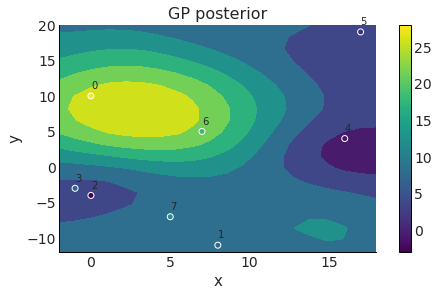
\includegraphics[width=\linewidth]{img/schools_gp_posterior}
    \end{column}
\end{columns}
\end{frame}
\begin{frame}[allowframebreaks]
\frametitle{References}
\bibliographystyle{abbrv}
\bibliography{../../../references.bib}
\end{frame}
\end{document}
% https://arxiv.org/pdf/0911.5367.pdf